\documentclass[a4paper,12pt]{article} % This defines the style of your paper
\usepackage[top = 2.5cm, bottom = 2.5cm, left = 2.5cm, right = 2.5cm]{geometry} 
\usepackage[T1]{fontenc}
\usepackage[utf8]{inputenc}
\usepackage{multirow} % Multirow is for tables with multiple rows within one cell.
\usepackage{booktabs} % For even nicer tables.
\usepackage{graphicx} 
\usepackage[spanish]{babel}
\usepackage{enumitem}
\usepackage{setspace}
\setlength{\parindent}{0in}
\usepackage{float}
\usepackage{fancyhdr}
\usepackage{caption} 
\usepackage{xcolor}      % Para los colores
\usepackage{fancyvrb}    % Para el entorno Verbatim personalizado
\usepackage{enumitem} %personalizar los enumarates
\usepackage{setspace}

% Definimos un nuevo entorno Verbatim llamado MyVerbatim
	\DefineVerbatimEnvironment{MyVerbatim}{Verbatim}
	{formatcom=\color{blue}}  % Aquí puedes cambiar el color
%%%%%%%%%%%%%%%%%%%%%%%%%%%%%%%%%%%%%%%%%%%%%%%%
% 3. Header (and Footer)
%%%%%%%%%%%%%%%%%%%%%%%%%%%%%%%%%%%%%%%%%%%%%%%%

\pagestyle{fancy} % With this command we can customize the header style.

\fancyhf{} % This makes sure we do not have other information in our header or footer.

\lhead{\footnotesize EST526: Introducción a la Estadística No Paramétrica}% \lhead puts text in the top left corner. \footnotesize sets our font to a smaller size.

%\rhead works just like \lhead (you can also use \chead)
\rhead{\footnotesize Rodríguez-Flores, Zayner Edin} %<---- Fill in your lastnames.

% Similar commands work for the footer (\lfoot, \cfoot and \rfoot).
% We want to put our page number in the center.
\cfoot{\footnotesize \thepage} 
\captionsetup[figure]{labelfont=bf} % Configura los captions de las figuras
\captionsetup[table]{labelfont=bf}  % Configura los captions de las tablas
	\begin{document}
		

		\thispagestyle{empty} % This command disables the header on the first page. 
		
		\begin{tabular}{p{15.5cm}} % This is a simple tabular environment to align your text nicely 
			{\large \bf EST 526 Introducción a la Estadística No Paramétrica} \\
			Zayner Edin Rodríguez Flores \\ Postgrado en Edafología  \\ Colegio de Postgraduados-Campus Montecillo\\
			\hline % \hline produces horizontal lines.
			\\
		\end{tabular} % Our tabular environment ends here.
		
		\vspace*{0.3cm} % Now we want to add some vertical space in between the line and our title.
		
		\begin{center} % Everything within the center environment is centered.
			{\Large \bf Tarea 1} % <---- Don't forget to put in the right number
			\vspace{2mm}
			
			% YOUR NAMES GO HERE
			{\bf Prueba de signos de \textit{Wilcoxon}, Rangos con signos, Prueba de \textit{t}, Prueba de \textit{Mann Withney} } % <---- Fill in your names here!
			
		\end{center}  
\vspace{0.4 cm}

		Para la realización de esta tarea los ejercicios se realizaron en el entorno RStudio para el lenguaje de programación R.
		\section*{Problema 1} 
		Pruebe la hipótesis nula de que la mediana de los flujos anuales para el el rio Conecuh en Brantley, Alabama es 683 pies cúbicos por segundo (cfs) para el periodo de 1941 - 1960. La hipótesis alternativa es que es inferior a 683 cfs.\\
		\begin{table}[H]
			\centering
			\begin{tabular}{|c|c|} \hline
				\textbf{Year}&\textbf{Flow (cfs)} \\ \hline
				1941&369\\
				1942&683\\
				1943&923\\
				1944&1193\\
				1945&413\\
				1946&1025\\
				1947&894\\
				1948&859\\
				1949&1157\\
				1950&524\\
				1951&327\\
				1952&574\\
				1953&762\\
				1954&578\\
				1955&379\\
				1956&374\\
				1957&581\\
				1958&581\\
				1959&530\\
				1960&929\\\hline
			\end{tabular}
			\caption{Flujos anuales para el rio \textit{Conecuh}}
			\label{tab:my_label}
		\end{table}
		\newpage
\begin{enumerate} [label=\textbf{\alph*})]
			\item {Establezca el Juego de Hipótesis} 
			\begin{center}
				Ho=Mediana=683\\
				Ha=Mediana<683
			\end{center}
			
			\item {Realice una gráfica de caja (Boxplot)} 
			
			\begin{MyVerbatim}
# Cargar librerias #
library(ggplot)
library(ggthemes)

# Cargar datos #
river<-read.csv("river.csv",header = TRUE)
Flujo<-river$Flow
		
 Generar el boxplot #
ggplot(river, aes(y = Flujo)) +
geom_boxplot(fill = "orange", color = "blue") +
labs(title = "Boxplot de Flujos Anuales para el Río Conecuh",
y = "Flujo (cfs)") +
theme_calc()
		\end{MyVerbatim}
			
\begin{figure}[H]
	\centering
	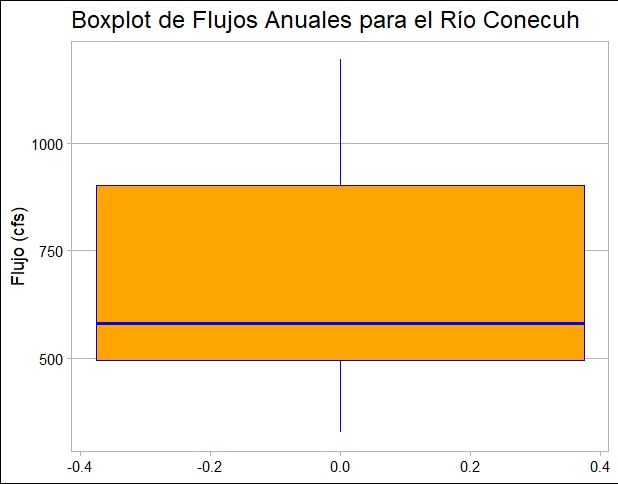
\includegraphics[width=0.7\linewidth]{Box_1}
	\captionsetup{labelfont=bf}
	\caption[Boxplot del Flujo del Rio Conecuh]{Boxplot del Flujo del Rio Conecuh}
	\label{fig:box1}
\end{figure}
			\item {Utilice la prueba del signo para probar la hipotesis en a) usando un \( \alpha = 0.05 \). Concluya }
			
			\begin{MyVerbatim}
# Prueba del signo #
binom.test(8,19,.5,alternative="less")
			\end{MyVerbatim}
			Resultando:
			
			\begin{MyVerbatim}
			
		Exact binomial test
			
data:  8 and 19
number of successes = 8, number of trials = 19,
p-value = 0.3238
alternative hypothesis: true probability of success is less than 0.5
95 percent confidence interval:
0.0000000 0.6318848
sample estimates:
probability of success 
0.4210526
				\end{MyVerbatim}
		\item {Utilice la prueba de Rangos con signos de Wilcoxon para probar la hipótesis en a) usando un \( \alpha = 0.05 \).
					Concluya.}
					\begin{MyVerbatim}
 	# Prueba de rangos de Wilcoxon #
wilcox.test(Flujo,mu=683,alternative="less")
					\end{MyVerbatim}
				Resultando:
				
				\begin{MyVerbatim}
	Wilcoxon signed rank test with continuity correction
					
data:  Flujo
V = 92, p-value = 0.4599
alternative hypothesis: true location is less than 683
				\end{MyVerbatim}
	   	\item {Utilice la prueba de t para probar la hipótesis en a) usando un  \( \alpha = 0.05 \) . Verifique supuesto de normalidad, Concluya.}
			\begin{MyVerbatim}
	# Prueba de t #
				
t.test(Flujo, mu = 683, alternative = "less")
				
			\end{MyVerbatim}
			Resultando: 
			\begin{MyVerbatim}
	One Sample t-test
				
data:  Flujo
t = -0.0041483, df = 19, p-value = 0.4984
alternative hypothesis: true mean is less than 683
95 percent confidence interval: -Inf 786.9568
sample estimates: mean of x  682.75 ..
\end{MyVerbatim}
Prueba de normalidad (QQPlot):
			\begin{MyVerbatim}
	# Gráfica QQplot de Flujo # 
				
ggplot(river, aes(sample = Flujo)) +
stat_qq() +
stat_qq_line() +
labs(title = "QQplot de Flujos Anuales para el Río Conecuh",
x = "Cuantiles Teóricos",
y = "Cuantiles Observados") +
theme_calc()
\end{MyVerbatim}
Resultado:
\begin{figure}[H]
	\centering
	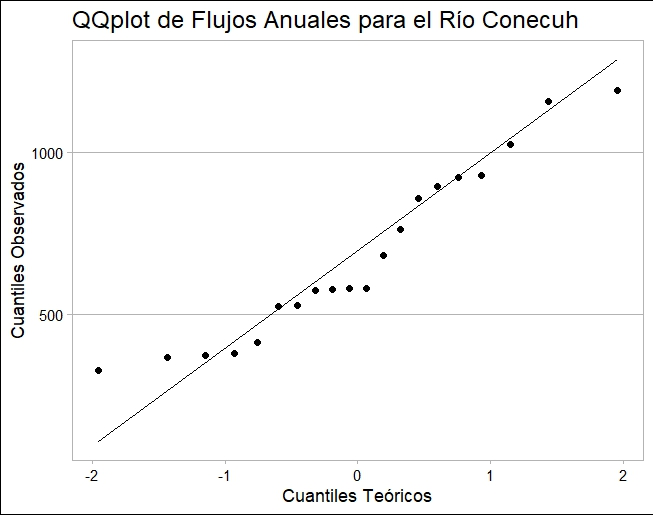
\includegraphics[width=0.7\linewidth]{qqplot}
	\captionsetup{labelfont=bf}
	\caption[qqplot]{Gráfico Q-Q Plot, de normalidad para la variable Flujo.}
	\label{fig: Gráfico qqplot, de normalidad para la variable Flujo}
\end{figure}
\begin{MyVerbatim}
	# Prueba de Shapiro-Wilk  #
shapiro.test(Flujo)
\end{MyVerbatim}
Resultado:
\begin{MyVerbatim}
	
	Shapiro-Wilk normality test
	
data:  Flujo
W = 0.92706, p-value = 0.1356
\end{MyVerbatim}
De acuerdo con las pruebas anterior y la representación gráfica (Figura 1) se puede concluir que no se puede descartar la normalidad de los datos. Además de acuerdo con los criterios de la prueba de signos de Wilcoxon, no se rechaza la Ho.
		\end{enumerate}
		
		\clearpage
\section*{Problema 2}
Los siguientes valores de conductancia específica fueron medidos en las dos bifurcaciones del Río Shenandoah: en Virginia usa
\begin{center}
	\begin{table}[H]
		\centering
		\begin{tabular}{|c|c|c|} \hline
			\textbf{Date}&\textbf{South Fork}&\textbf{North Fork}\\ \hline
			5-23-83&194&255\\
			8-16-83&348&353\\
			10-05-83&383&470\\
			11-15-83&225&353\\
			1-10-84&266&353\\
			2-22-84&194&295\\
			4-24-84&212&199\\
			6-04-84&320&410\\
			7-19-84&340&346\\
			8-28-84&310&405\\ \hline
			\end{tabular}
			\caption{Conductancia especifica de dos bifurcaciones del río Shenandosh, Virginia, USA}
			\label{tab:my_label2}
		\end{table}
	\end{center}
	\begin{enumerate} [label=\textbf{\alph*})]
		\item { Enuncie las hipótesis nula y alterna apropiadas para ver si los valores de conductancia son lo mismo en las dos bifurcaciones del rio.}\\
			\begin{center}
			Ho: North Fork = South Fork\\
			Ha: \(North Fork \neq South Fork\)
		\end{center}
		\item {Ilustre y verifique los resultados con una gráfica.}
\begin{MyVerbatim}
	# Boxplot de North
a<-ggplot(conductancia, aes(y = North)) +
geom_boxplot(fill = "orange", color = "blue") +
labs(title = "Boxplot de Conductancia de Sur",
y = "Conductancia") +
theme_calc()
	# Boxplot de South
b<-ggplot(conductancia, aes(y = South)) +
geom_boxplot(fill = "orange", color = "blue") +
labs(title = "Boxplot de Conductancia de Norte",
y = "Conductancia") +
theme_calc()
	# Juntar graficas
combined_plots <- a + b
combined_plots
\end{MyVerbatim}
\begin{figure}[H]
	\centering
	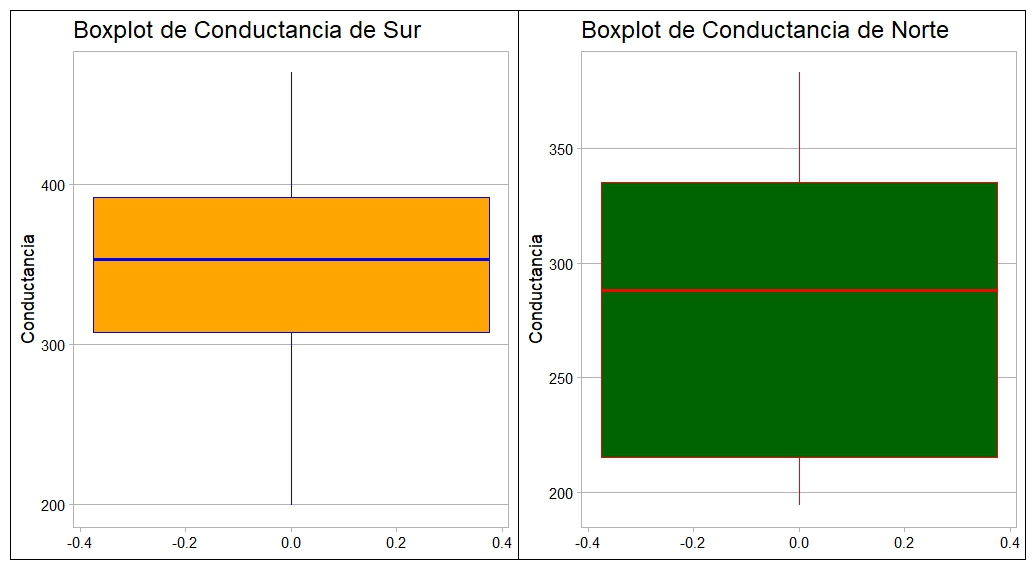
\includegraphics[width=0.7\linewidth]{2Box}
	\caption[2Box]{Boxplot de conductancia Norte y Sur}
	\label{fig:2box}
\end{figure}
\item {Realice la prueba del signo para muestras pareadas usando un \( \alpha = 0.05 \). Concluya.}
	\begin{MyVerbatim}
	# Prueba del signo #
binom.test(9,10,.5,alternative="two.sided")
	\end{MyVerbatim}
Resultando:
\begin{MyVerbatim}
	Exact binomial test
	
data:  9 and 10
number of successes = 9, number of trials = 10, p-value = 0.02148
alternative hypothesis: true probability of success is not equal to 0.5
95 percent confidence interval: 0.5549839 0.9974714
sample estimates: probability of success  0.9 
	
\end{MyVerbatim}

\item {Utilice las diferencias y la prueba de Rangos con signos de \textit{Wilcoxon} para probar la hipótesis en a) usando un \( \alpha = 0.05 \). Concluya.}
\begin{MyVerbatim}
	# Prueba de rangos con signos de Wilcoxon##
North<-conductancia$North
South<-conductancia$South
wilcox.test(South, North, paired = TRUE, alternative = "two.sided")
data.frame(South, North)
\end{MyVerbatim}
Resultado:
\begin{MyVerbatim}

	Wilcoxon signed rank test with continuity correction

data:  South and North
V = 3, p-value = 0.01437
alternative hypothesis: true location shift is not equal to 0
\end{MyVerbatim}

\item {Trate de realizar la comparación de las conductancias en ambos brazos usando una prueba t para muestras pareadas.}
\begin{MyVerbatim}
	# Prueba de t #
t.test(South,North, paired = TRUE, alternative = "two.sided")
\end{MyVerbatim}
Resultado:
\begin{MyVerbatim}
	Paired t-test
	
data:  South and North
t = -4.2419, df = 9, p-value = 0.002168
alternative hypothesis: true mean difference is not equal to 0
95 percent confidence interval: -99.20406 -30.19594
sample estimates: mean difference -64.7 
\end{MyVerbatim}
Dado que las medianas son diferentes (p-value: 0.002168 < \( \alpha = 0.05 \)), se rechaza la Ho. 
\item {¿Por qué los resultados son similares o diferentes?}\\
\\
Los resultados son similares dado que cada una de las pruebas realizadas los valores de p-value son menor al valor de \( \alpha = 0.05 \)), por lo que en ambos casos se rechaza la Ho.

\item {Estime la cantidad por la cual las bifurcaciones difieren en conductancia, independientemente de la prueba.}
\begin{MyVerbatim}
	# Diferencia de medias #
# Calcular las diferencias absolutas #
differences <- abs(South - North)
	
# Calcular la media de las diferencias absolutas #
mean_difference <- mean(differences)
mean_difference
[1] 67.3
\end{MyVerbatim}
De acuerdo con las diferencias absolutas entre ambas bifurcaciones, se puede estimar un valor de 67.3 de promedio en las diferencias de cada observación.
	\end{enumerate}
\newpage
\section*{Problema 3}
La respiración del suelo es una medida de la actividad microbiana en el suelo, que afecta el crecimiento de las plantas. En un estudio, se tomaron muestras de suelo de dos ubicaciones en un bosque: 1) debajo de una abertura en el dosel del bosque (la ubicación de “brecha”) y 2) en un área cercana bajo un crecimiento denso de árboles (la ubicación de “crecimiento”). Se midió la cantidad de dióxido de carbono emitido por cada muestra de suelo (en mol CO2/g de suelo/h). La cuestión es probar si las áreas de brecha y crecimiento no difieren con respecto a la respiración del suelo.
\begin{center}
	\begin{table}[H]
	\centering
	\begin{tabular}{|c|c|} \hline
		\textbf{Condition}&\textbf{Respiration} \\ \hline
		growth&17\\
		growth&20\\
		growth&170\\
		growth&315\\
		growth&22\\
		growth&190\\
		growth&64\\
		gap&22\\
		gap&29\\
		gap&13\\
		gap&16\\
		gap&15\\
		gap&18\\
		gap&15\\
		gap&6\\ \hline
	\end{tabular}
	\caption{Respiración del suelo en dos diferentes condiciones}
	\label{tab:my_label3}
\end{table}
\end{center}
\begin{enumerate} [label=\textbf{\alph*})]
\item Establezca el juego de hipótesis para este caso.
\begin{center}
	Ho: Áreas de brecha = Crecimiento\\
	Ha: \(Áreas de brecha \neq Crecimiento\)
\end{center}
\item Grafique los datos usando boxplot
\begin{MyVerbatim}
	# Gráfica Boxplot #
ggplot(Ejercicio.3, aes(x=Condicion, y=Respiracion)) 
+ geom_boxplot(fill = "orange", color = "blue") 
+ theme_calc()
\end{MyVerbatim}
Resultado: 
\begin{figure} [H]
	\centering
	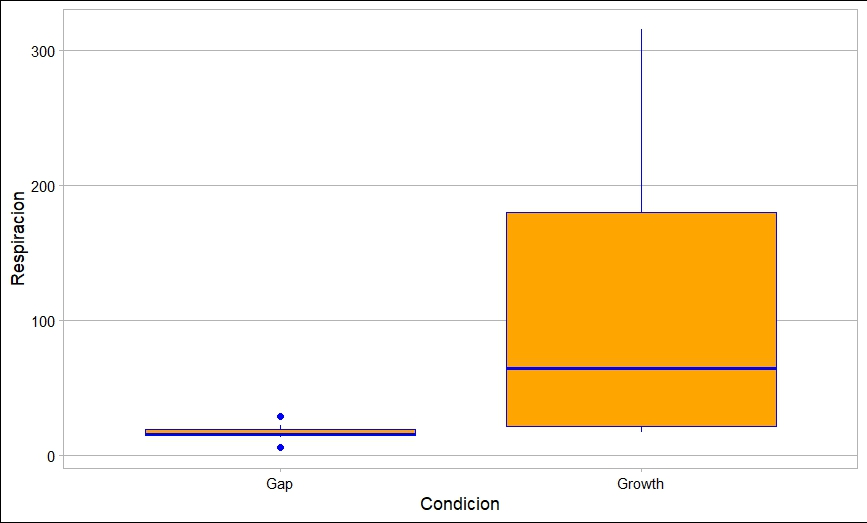
\includegraphics[width=0.7\linewidth]{condic}
	\caption{Respiración bajo distintos tios de condición de crecimiento}
	\label{fig:condic}
\end{figure}
\item Utilice la prueba de Mann Withney usando un  \( \alpha = 0.05 \). Concluya.
\begin{MyVerbatim}
	# Mann Withney #
Ejercicio.3$Condicion=as.factor(Ejercicio.3$Condicion)
wilcox.test(Respiracion~Condicion, data=Ejercicio.3)
\end{MyVerbatim}
Resultado:\\ 
De acuerdo a los resultados de la prueba anterior (p-value: 0.01491 < 0.05), se rechaza la Ho con un 95\% de confiabilidad
\item Utilice una prueba de t para poblaciones independientes suponiendo homogeneidad de varianzas. Use un \(\alpha=0.05\). Verifique normalidad.
\begin{MyVerbatim}
	# Prueba de t paramétrica #
t.test(Respiracion~Condicion, data=Ejercicio.3)
\end{MyVerbatim}
Resultado:\\
\begin{MyVerbatim}
	Welch Two Sample t-test

data:  Respiracion by Condicion
t = -2.2458, df = 6.0362, p-value = 0.06556
alternative hypothesis: true difference in means between group Gap 
and group Growth is not equal to 0
95 percent confidence interval: -203.056476    8.556476
sample estimates: 
mean in group Gap mean in group Growth 
16.75               114.00
\end{MyVerbatim}
Suponiendo normalidad, se realizara una ANOVA:
\begin{MyVerbatim}
	# ANOVA #
Resultado<-aov(Respiracion~Condicion, data=Ejercicio.3)
anova(Resultado)
\end{MyVerbatim}
Resultado:\\
\begin{MyVerbatim}
	Analysis of Variance Table

Response: Respiracion
Df Sum Sq Mean Sq F value  Pr(>F)  
Condicion  1  35308   35308  5.8222 0.03132 *
Residuals 13  78838    6064                  
---
Signif. codes:  0 ‘***’ 0.001 ‘**’ 0.01 ‘*’ 0.05 ‘.’ 0.1 ‘ ’ 1
\end{MyVerbatim}
Prueba de normalidad:\\
\begin{MyVerbatim}
	# Prueba de normalidad
resid<-resid(Resultado)
shapiro.test(resid)
\end{MyVerbatim}
Resultado: \\
	\begin{MyVerbatim}
	Shapiro-Wilk normality test
		
data:  resid
W = 0.86346, p-value = 0.02708	
	\end{MyVerbatim}
\item ¿Cuál prueba recomienda?\\
De acuerdo a la prueba de normalidad, y que el valor p-value es inferior a 0.05. La recomendación seria realizar la prueba de Mann Withney ya que los datos no cumplen con el supuesto de normalidad.
\end{enumerate}
\newpage
\section*{Problema 4}
Para este caso utilizamos los mismos datos de fitorremediación que para la prueba t de dos muestras. Recordemos que la fitorremediación es el uso de plantas para remediar suelos y aguas contaminados, y que las especies vegetales se seleccionan en función de su capacidad para absorber o estabilizar contaminantes específicos en un lugar.\\
Aquí estudiaremos la eficacia de dos plantas de cultivo (remolacha roja y cebada) para eliminar el cadmio de los 20 cm superiores del suelo en un lugar contaminado. Los datos que tenemos son el porcentaje de reducción de cadmio después de una cosecha.\\
Como sólo tenemos 15 observaciones para cada planta, decidimos utilizar una prueba no paramétrica. Como tenemos dos muestras independientes, utilizamos una prueba de Mann-Whitney para dos muestras.
\begin{enumerate} [label=\textbf{\alph*})]
	\item Pruebe la hipótesis nula de que no existe diferencia en la efectividad de Redbeet y Barley para remover Cadmio en los primeros 20 cm de profundidad.\\
	
	\begin{center}
		Juego de Hipótesis:\\
		Ho= MeRedbeet= MeBarley\\
		Ha=\(MeRedbeet \neq MeBarley)\)\\
	\end{center}
	\begin{MyVerbatim}
# Datos #
redbeet <- c(18, 5, 10, 8, 16, 12, 8, 8, 11, 5, 6, 8, 9, 21, 9)
barley <- c(8, 5, 10, 19, 15, 18, 11, 8, 9, 4, 5, 13, 7, 5, 7)

wilcox.test(redbeet,barley, 
alternative = "two.sided", conf.int = TRUE, conf.level = 0.95)

		
wilcox.test(Cd.BeetBarley$redbeet, Cd.BeetBarley$barley, 
alternative = "two.sided", conf.int = TRUE, conf.level = 0.95)
	\end{MyVerbatim}
Resultado:\\
\begin{MyVerbatim}
Wilcoxon rank sum test with continuity correction

data:  redbeet and barley
W = 126.5, p-value = 0.5728
alternative hypothesis: true location shift is not equal to 0
95 percent confidence interval: -2.000012  3.999994
sample estimates:
difference in location  0.9999553 
\end{MyVerbatim}
De acuerdo a los resultados anteriores se puede concluir que no existe diferencia estadistica entre ambos casos de fitorremediacion por lo que se no se rechaza la Ho de que ambas medianas son similares.
\end{enumerate}
\end{document}
